\section{Problem Definition}

\begin{figure}[t]
\centering
\begin{subfigure}[b]{0.3\textwidth}
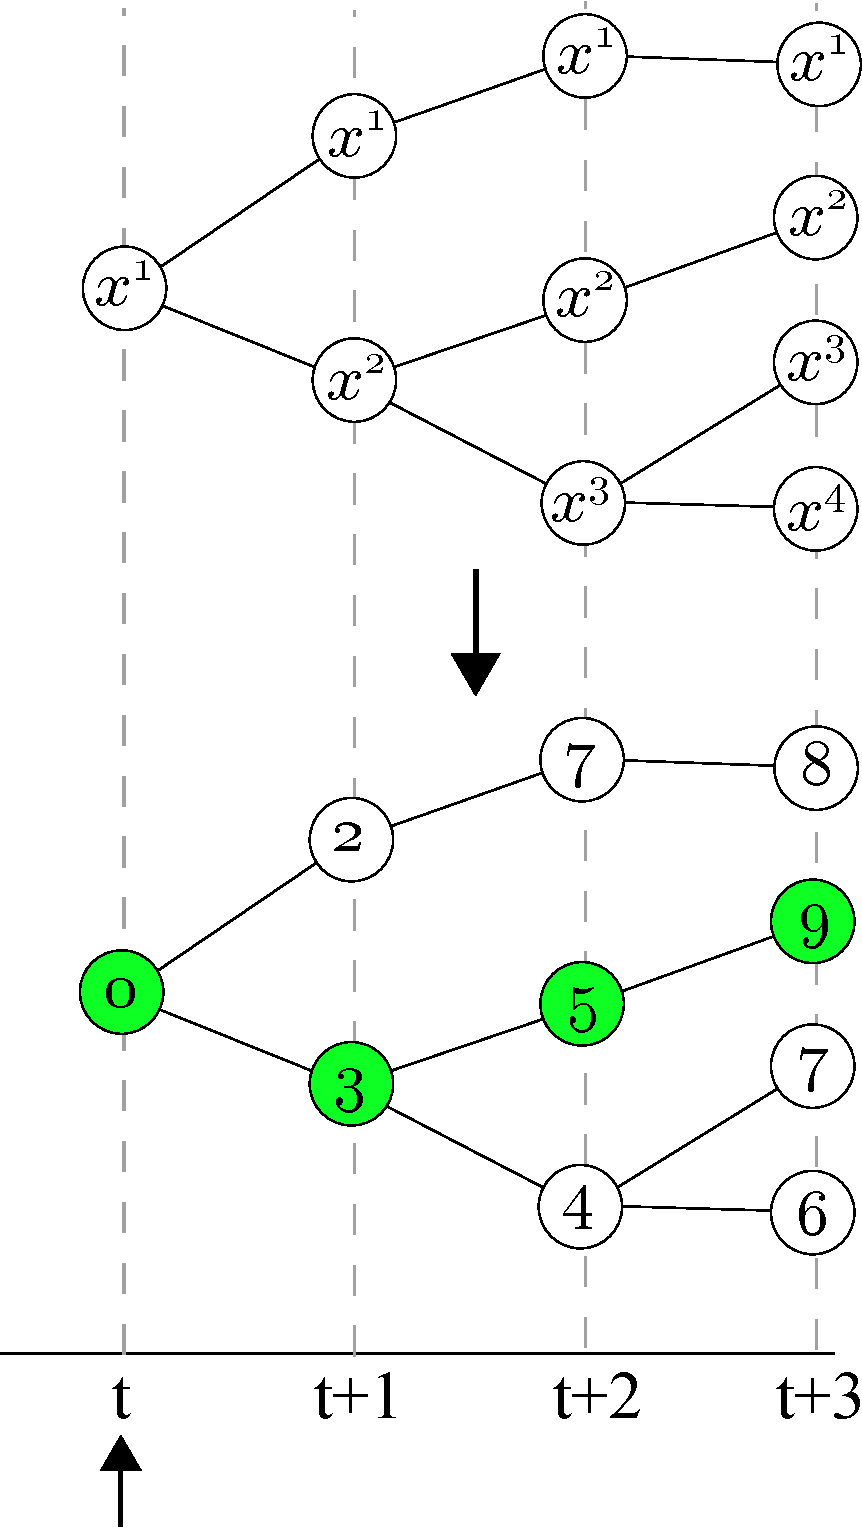
\includegraphics[height=3in]{plan_at_t0}
\caption{A gull}
\label{fig:plan_at_t0}
\end{subfigure}
\hspace{1in}
\begin{subfigure}[b]{0.3\textwidth}
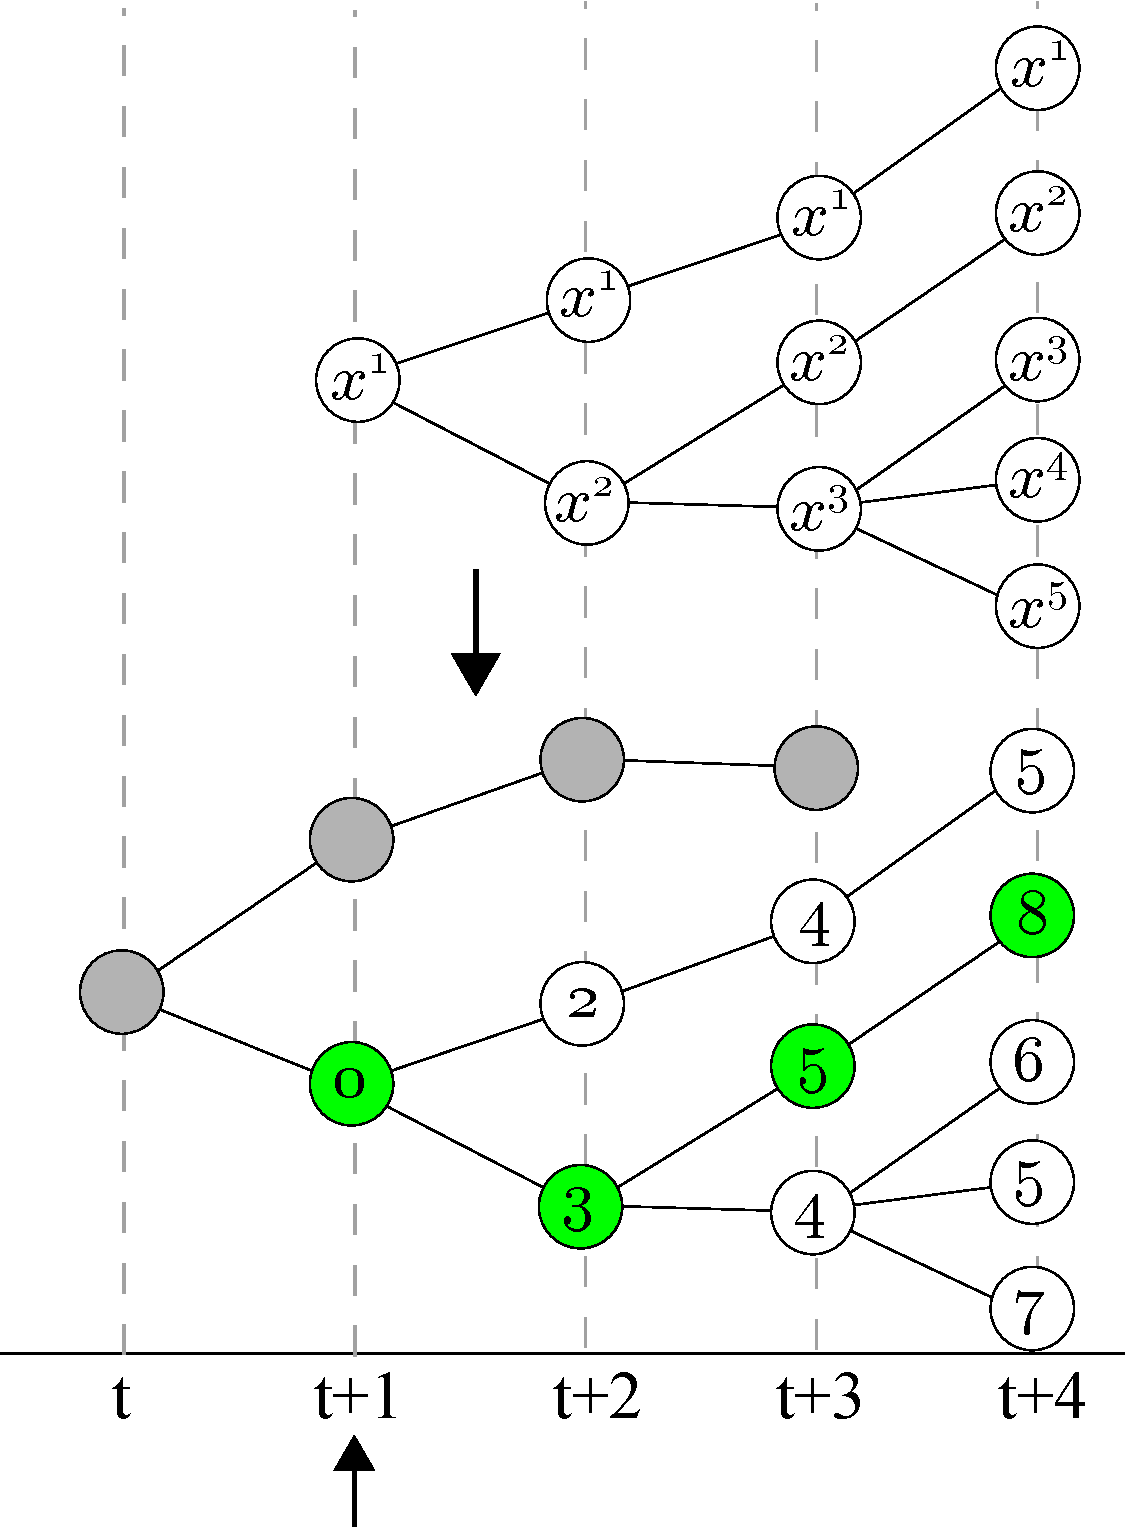
\includegraphics[height=3in]{plan_at_t1}
\caption{A mouse}
\label{fig:plan_at_t1}
\end{subfigure}%

\end{figure}


Our goal is to enable receding horizon planning for active SLAM in a computationally tractable formulation. The active SLAM exploration problem can be framed as determining the control actions which guide a robot to a state that maximizes mutual information between its current and future maps. We model the environment as an occupancy grid map, and represent the map as a conglomeration of cells: $m = \{m^{i}\}_{i=1}^{N}$. The probability that an individual cell is occupied at $t$ is given by $p\left(m^{i} \ \vert \ x_{1:t}, z_{1:t}\right)$, where $x_{1:t}$ denotes the history of states of the vehicle, and $z_{1:t}$ denotes the history of range observations accumulated by the vehicle. Additionally we assume that cell occupancies  are independent of one another: $p\left(m \ \vert \ x_{1:t}, z_{1:t}\right) = \prod_{i} p\left(m^{i} \ \vert \ x_{1:t}, z_{1:t}\right)$. For notational simplicity we write the map conditioned on random variables $x_{1:t}$ and $z_{1:t}$ as $p\left(m_{t}\right) \equiv p\left(m \ \vert \ x_{1:t}, z_{1:t}\right)$.

The optimal plan over a one step horizon will guide the robot to a state, $x_{t+1}^{*}$, in which the mutual information between $m_{t}$ and $m_{t+1}$ is maximized.

\begin{align} \begin{split}
    x_{t+1}^{*}
    &=
    \argmax_{x_{t+1}}
    \
    \text{IG}\left[
        m_{t}
        ;
        m_{t+1}
    \right]
    \\
    &=
    \argmax_{x_{t+1}}
    \
    \text{H}\left[
        m_{t}
    \right]
    -
    \expect_{z_{t+1}}\left[
        \text{H}\left[
            m_{t+1}
        \right]
    \right]
    \\
    &=
    \argmin_{x_{t+1}}
    \
    \expect_{z_{t+1}}\left[
        \text{H}\left[
            m_{t+1}
        \right]
    \right]
\end{split} \end{align}

The term $\text{H}\left[m_{t}\right]$ is independent of the future state $x_{t+1}$, so the information gain is maximized when $x_{t+1}$ minimizes the expected entropy of the updated map. The independence between cell occupancies allows us to write the future entropy of the map as a sum of future entropies of individual grid cells:

\begin{align} \begin{split}
    \text{H}\left[
        m_{t+1}
    \right]
    &=
    \sum_{i=1}^{N}
    \text{H}\left[
        m_{t+1}^{i}
        \ \vert \
        m_{t+1}^{i-1}
        , \
        \dots
        \ ,
        m_{t+1}^{1}
    \right]
    \\
    &=
    \sum_{i=1}^{N}
    \text{H}\left[
        m_{t+1}^{i}
    \right]
\end{split} \end{align}

The expectation to minimize is therefore

\begin{align} \begin{split}
    \expect_{z_{t+1}}\left[
        \text{H}\left[
            m_{t+1}
        \right]
    \right]
    &=
    \int
    p\left(
        z_{t+1}
    \right)
    \sum_{i=1}^{N}
    \text{H}\left[
        m_{t+1}^{i}
    \right]
    dz_{t+1}
    \\
    &=
    -\expect_{z_{t+1}}\left[
        \sum_{i=1}^{N}
        \log p\left(
            m_{t+1}^{i}
        \right)
    \right]
\end{split} \end{align}
